% Options for packages loaded elsewhere
\PassOptionsToPackage{unicode}{hyperref}
\PassOptionsToPackage{hyphens}{url}
\PassOptionsToPackage{dvipsnames,svgnames,x11names}{xcolor}
%
\documentclass[
  12pt,
  letterpaper,
  egregdoesnotlikesansseriftitles]{scrreprt}

\usepackage{amsmath,amssymb}
\usepackage{iftex}
\ifPDFTeX
  \usepackage[T1]{fontenc}
  \usepackage[utf8]{inputenc}
  \usepackage{textcomp} % provide euro and other symbols
\else % if luatex or xetex
  \usepackage{unicode-math}
  \defaultfontfeatures{Scale=MatchLowercase}
  \defaultfontfeatures[\rmfamily]{Ligatures=TeX,Scale=1}
\fi
\usepackage{lmodern}
\ifPDFTeX\else  
    % xetex/luatex font selection
  \setmainfont[]{Palatino Linotype}
\fi
% Use upquote if available, for straight quotes in verbatim environments
\IfFileExists{upquote.sty}{\usepackage{upquote}}{}
\IfFileExists{microtype.sty}{% use microtype if available
  \usepackage[]{microtype}
  \UseMicrotypeSet[protrusion]{basicmath} % disable protrusion for tt fonts
}{}
\makeatletter
\@ifundefined{KOMAClassName}{% if non-KOMA class
  \IfFileExists{parskip.sty}{%
    \usepackage{parskip}
  }{% else
    \setlength{\parindent}{0pt}
    \setlength{\parskip}{6pt plus 2pt minus 1pt}}
}{% if KOMA class
  \KOMAoptions{parskip=half}}
\makeatother
\usepackage{xcolor}
\setlength{\emergencystretch}{3em} % prevent overfull lines
\setcounter{secnumdepth}{5}
% Make \paragraph and \subparagraph free-standing
\ifx\paragraph\undefined\else
  \let\oldparagraph\paragraph
  \renewcommand{\paragraph}[1]{\oldparagraph{#1}\mbox{}}
\fi
\ifx\subparagraph\undefined\else
  \let\oldsubparagraph\subparagraph
  \renewcommand{\subparagraph}[1]{\oldsubparagraph{#1}\mbox{}}
\fi


\providecommand{\tightlist}{%
  \setlength{\itemsep}{0pt}\setlength{\parskip}{0pt}}\usepackage{longtable,booktabs,array}
\usepackage{calc} % for calculating minipage widths
% Correct order of tables after \paragraph or \subparagraph
\usepackage{etoolbox}
\makeatletter
\patchcmd\longtable{\par}{\if@noskipsec\mbox{}\fi\par}{}{}
\makeatother
% Allow footnotes in longtable head/foot
\IfFileExists{footnotehyper.sty}{\usepackage{footnotehyper}}{\usepackage{footnote}}
\makesavenoteenv{longtable}
\usepackage{graphicx}
\makeatletter
\def\maxwidth{\ifdim\Gin@nat@width>\linewidth\linewidth\else\Gin@nat@width\fi}
\def\maxheight{\ifdim\Gin@nat@height>\textheight\textheight\else\Gin@nat@height\fi}
\makeatother
% Scale images if necessary, so that they will not overflow the page
% margins by default, and it is still possible to overwrite the defaults
% using explicit options in \includegraphics[width, height, ...]{}
\setkeys{Gin}{width=\maxwidth,height=\maxheight,keepaspectratio}
% Set default figure placement to htbp
\makeatletter
\def\fps@figure{htbp}
\makeatother


% Wird für die Tabelle im Titelblatt der Experten verwendet:
% Array
\usepackage{array}
% Neue Definition für Tabelleneinträge
% linksbündig mit Breitenangabe
\newcolumntype{L}[1]{>{\raggedright\arraybackslash}p{#1}} 
% zentriert mit Breitenangabe
\newcolumntype{C}[1]{>{\centering\arraybackslash}p{#1}} 
% rechtsbündig mit Breitenangabe
\newcolumntype{R}[1]{>{\raggedleft\arraybackslash}p{#1}} 

\usepackage[a4paper, margin=3cm]{geometry}

% Change math font





\makeatletter
\@ifpackageloaded{bookmark}{}{\usepackage{bookmark}}
\makeatother
\makeatletter
\@ifpackageloaded{caption}{}{\usepackage{caption}}
\AtBeginDocument{%
\ifdefined\contentsname
  \renewcommand*\contentsname{Inhaltsverzeichnis}
\else
  \newcommand\contentsname{Inhaltsverzeichnis}
\fi
\ifdefined\listfigurename
  \renewcommand*\listfigurename{Abbildungsverzeichnis}
\else
  \newcommand\listfigurename{Abbildungsverzeichnis}
\fi
\ifdefined\listtablename
  \renewcommand*\listtablename{Tabellenverzeichnis}
\else
  \newcommand\listtablename{Tabellenverzeichnis}
\fi
\ifdefined\figurename
  \renewcommand*\figurename{Abbildung}
\else
  \newcommand\figurename{Abbildung}
\fi
\ifdefined\tablename
  \renewcommand*\tablename{Tabelle}
\else
  \newcommand\tablename{Tabelle}
\fi
}
\@ifpackageloaded{float}{}{\usepackage{float}}
\floatstyle{ruled}
\@ifundefined{c@chapter}{\newfloat{codelisting}{h}{lop}}{\newfloat{codelisting}{h}{lop}[chapter]}
\floatname{codelisting}{Listing}
\newcommand*\listoflistings{\listof{codelisting}{Listingverzeichnis}}
\makeatother
\makeatletter
\makeatother
\makeatletter
\@ifpackageloaded{caption}{}{\usepackage{caption}}
\@ifpackageloaded{subcaption}{}{\usepackage{subcaption}}
\makeatother
\ifLuaTeX
\usepackage[bidi=basic]{babel}
\else
\usepackage[bidi=default]{babel}
\fi
\babelprovide[main,import]{ngerman}
\ifPDFTeX
\else
\babelfont{rm}[]{Palatino Linotype}
\fi
% get rid of language-specific shorthands (see #6817):
\let\LanguageShortHands\languageshorthands
\def\languageshorthands#1{}
\ifLuaTeX
  \usepackage{selnolig}  % disable illegal ligatures
\fi
\usepackage{bookmark}

\IfFileExists{xurl.sty}{\usepackage{xurl}}{} % add URL line breaks if available
\urlstyle{same} % disable monospaced font for URLs
\hypersetup{
  pdftitle={Tragverhalten von Stahlbetontragwerken},
  pdfauthor={Pascal Gitz},
  pdflang={de},
  colorlinks=true,
  linkcolor={Black},
  filecolor={Maroon},
  citecolor={Blue},
  urlcolor={Blue},
  pdfcreator={LaTeX via pandoc}}

% TITELBLATT, VERSIONSTABELLE UND SELBSTSTÄNDIGKEITSERKLÄRUNG
%--------------------------------------------------------------------------------------------------------------------


\titlehead{\includegraphics[height=0.5cm]{../imgs/logos/logo-mse}\hfill\includegraphics[height=0.5cm]{../imgs/logos/logo-hslu-en-col} \\ }
\subject{MASTER OF SCIENCE IN ENGINEERING\\Vertiefungsmodul I}
\title{Tragverhalten von Stahlbetontragwerken}

\subtitle
{Verformungsberechnungen mittels Finiten Elementen}

%\thanks{
%Version 1.0
%\hfill \today
%\hfill Hun}


\date{\large Horw, Freitag, 14. Juni 2024}
\author{Pascal Gitz}

\publishers{
	\begin{table}[H]
		\centering
		\begin{tabular}{L{2cm} L{6cm}}
			Advisor: & Prof. FH, Dr. Daniel Heinzmann \\
			Experte: & Dr. Thomas Jäger \\
		\end{tabular}
	\end{table}
}
\begin{document}
\maketitle


Hiermit erkläre ich, dass ich die vorliegende Arbeit selbstständig angefertigt und keine anderen als die angegebenen Hilfsmittel verwendet habe. Sämtliche verwendeten Textausschnitte, Zitate oder Inhalte anderer Verfasser wurden ausdrücklich als solche gekennzeichnet.\\%
%
\\%
%
Horw, 19. Januar 2024 \hfill Pascal Gitz%

\vfill
%\begin{tabular}[h]{llcr} 
    %*Version 2.0 & - Definitives Exemplar & \today & MK \\ 
    %*Version 1.0 & - Prüfungsexemplar & 22. Januar 2021 & MK \\ 
%\end{tabular}\\

% Version 2.0 - Definitives Exemplar \hfill \today \quad \quad \quad \quad \quad MK\\
Version 1.0 - Prüfungsexemplar \hfill 19. Januar 2024 \quad \quad \quad \quad \quad PG\\
Version 0.9 - Entwurf \hfill 08. Januar 2024 \quad \quad \quad \quad \quad PG\\

\newpage

\chapter*{Kurzfassung}

-

\renewcommand*\contentsname{Inhaltsverzeichnis}
{
\hypersetup{linkcolor=}
\setcounter{tocdepth}{1}
\tableofcontents
}
\listoffigures
\listoftables
\bookmarksetup{startatroot}

\chapter{Einleitung}\label{einleitung}

\begin{itemize}
\tightlist
\item
\end{itemize}

\bookmarksetup{startatroot}

\chapter{Modelle mit Drehfedern}\label{modelle-mit-drehfedern}

\section{Nachrechnung Kragarm}\label{nachrechnung-kragarm}

Um das Verhalten der FE-Programme mit Drehfedern einzuschätzen, werden
Verformungen an einem fiktivem Beispiel bestimmt. Dargestellt ist der
Kragarm in Abbildung~\ref{fig-kragarm-feder}. Die Verformung an der
Stelle \(w\) wird händisch mittels Arbeitsgleichung und mit dem
FE-Programm bestimmt. Es sollen nicht-lineare Federsteifigikeiten
berücksichtigt werden können.

\begin{figure}[H]

\centering{

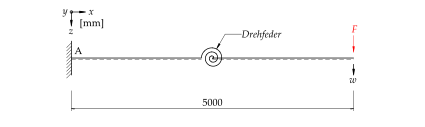
\includegraphics{index_files/mediabag/../imgs/Kragarm_system_Feder.pdf}

}

\caption{\label{fig-kragarm-feder}Statisches System des Kragarms}

\end{figure}%

Die Parameter in der Tabelle~\ref{tbl-parameters-kragarm} dienen als
Berechnungsgrundlagen. Beschrieben sind die Abmessungen und
Materialeigenschaften, sowie die Beiden Laststufen \(F_1\) und \(F_2\)
wie auch die Federsteifigkeiten \(k_1\) und \(k_2\). Die Laststufen sind
so gewählt, dass das nicht-lineare Verhalten der Drehfeder zu tragen
kommt.

\begin{longtable}[]{@{}
  >{\raggedright\arraybackslash}p{(\columnwidth - 2\tabcolsep) * \real{0.5000}}
  >{\raggedright\arraybackslash}p{(\columnwidth - 2\tabcolsep) * \real{0.5000}}@{}}

\caption{\label{tbl-parameters-kragarm}Berechnungsparameter des
Kragarms}

\tabularnewline

\toprule\noalign{}
\begin{minipage}[b]{\linewidth}\raggedright
Parameter
\end{minipage} & \begin{minipage}[b]{\linewidth}\raggedright
\hspace{0pt}
\end{minipage} \\
\midrule\noalign{}
\endhead
\bottomrule\noalign{}
\endlastfoot
\(E = \frac{10000 \text{N}}{\text{mm}^{2}}\) &
\(F_{1} = - 10000 \text{N}\) \\
\(F_{2} = - 21500 \text{N}\) & \(b = 200 \text{mm}\) \\
\(h = 400 \text{mm}\) & \(k_{1} = \frac{100000 \text{N}}{\text{m}}\) \\
\(k_{2} = \frac{10000 \text{N}}{\text{m}}\) &
\(l_{Kragarm} = 5 \text{m}\) \\

\end{longtable}

Der Querschnitt ist in Abbildung~\ref{fig-qs-kragarm} aufgezeigt.

\begin{figure}[H]

\centering{

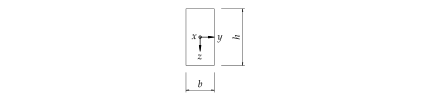
\includegraphics{index_files/mediabag/../imgs/Kragarm_querschnitt.pdf}

}

\caption{\label{fig-qs-kragarm}Fiktiver Querschnitt des Kragarms mit
linear-elastischem Materialverhalten}

\end{figure}%

Die Entsprechende Federcharakteristik ist in
Abbildung~\ref{fig-springcharacteristic} zu sehen.

\begin{figure}[H]

\centering{

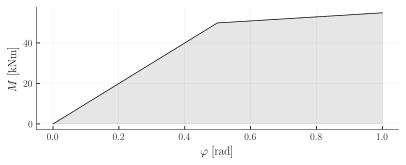
\includegraphics{index_files/mediabag/04_Kragarm_files/figure-pdf/fig-springcharacteristic-output-1.pdf}

}

\caption{\label{fig-springcharacteristic}Charakteristik der Drehfeder}

\end{figure}%

\subsection{Biegeverformung}\label{biegeverformung}

Apriori werden die Biegeverformungen mittels der Differentialgleichung
für reine Biegeträger ermittelt. Dabei wird die Drehfeder
vernachlässigt. Das statische System, gezeigt in
Abbildung~\ref{fig-kragarm-sys} führt zu den Zustandslinien der
Schnittgrössen in der \textbf{?@fig-sk-kragarmF1}.

\begin{figure}[H]

\centering{

\includegraphics{index_files/mediabag/../imgs/Kragarm_System.pdf}

}

\caption{\label{fig-kragarm-sys}Statisches System des Kragarms}

\end{figure}%

\begin{figure}[H]

\centering{

\includegraphics{index_files/mediabag/04_Kragarm_files/figure-pdf/fig-sk-kragarmf1-output-1.pdf}

}

\caption{\label{fig-sk-kragarmf1}Schnittkräfte des Systems aus
Abbildung~\ref{fig-kragarm-sys} für die Last \(F_1\)}

\end{figure}%

\begin{equation}w_{Bending,F1} = 39.06 \text{mm}\end{equation}

\begin{figure}[H]

\centering{

\includegraphics{index_files/mediabag/04_Kragarm_files/figure-pdf/fig-sk-kragarm-f2-output-1.pdf}

}

\caption{\label{fig-sk-kragarm-f2}Schnittkräfte des Systems aus
Abbildung~\ref{fig-kragarm-sys} für die Last \(F2\)}

\end{figure}%

\begin{equation}w_{Bending,F 2} = 83.98 \text{mm}\end{equation}

\subsection{Verformung der Drehfeder}\label{verformung-der-drehfeder}

Die Verformung aus der Drehfeder bedingt das Biegemoment des realen und
des fiktiven Systems an der Stelle der Drehfeder, sowie die
Federkonstante \(k_\varphi\). Das System is in
Abbildung~\ref{fig-kragarm-sys-virtuell} gezeigt.

\begin{figure}[H]

\centering{

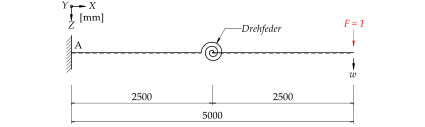
\includegraphics{index_files/mediabag/../imgs/Kragarm_system_feder_virtuell.pdf}

}

\caption{\label{fig-kragarm-sys-virtuell}Statisches System des Kragarms
im virtuellen Kräftezustand}

\end{figure}%

Die entsprechenden Verläufe der Querkraft und des Biegemoments in
Abbildung~\ref{fig-sk-kragarm-virtuell}.

\begin{figure}[H]

\centering{

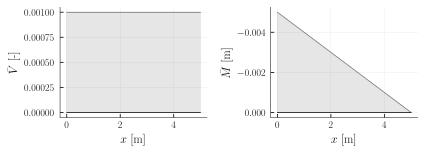
\includegraphics{index_files/mediabag/04_Kragarm_files/figure-pdf/fig-sk-kragarm-virtuell-output-1.pdf}

}

\caption{\label{fig-sk-kragarm-virtuell}Schnittkräfte des virtuellen
Systems aus Abbildung~\ref{fig-kragarm-sys-virtuell}}

\end{figure}%

Die Gleichung~\ref{eq-spring_rotation} berücksichtigt die zusätzliche
Verformung durch die Drehfeder.

\begin{equation}\phantomsection\label{eq-spring_rotation}{
w_{Spring} = \bar{M} \frac{M}{k_\varphi} = \bar{M} \varphi
}\end{equation}

Angewendet auf das System der Abbildung~\ref{fig-kragarm-feder} folgen
für die beiden Laststufen die Deformationen zu:

\begin{equation}w_{spring,F1} = 625.0 \text{mm}\end{equation}

\begin{equation}w_{spring,F2} = 2215.1 \text{mm}\end{equation}

\subsection{Vergleich mit FE}\label{vergleich-mit-fe}

\includegraphics{index_files/mediabag/04_Kragarm_files/figure-pdf/cell-14-output-1.pdf}

\begin{equation}w_{tot,F1} = 664.06 \text{mm}\end{equation}

\begin{figure}[H]

{\centering \includegraphics{../imgs/kragarm_fe_F1.png}

}

\caption{Verformungen in \(z\) Richtung mit FE für \(F_2\)}

\end{figure}%

\begin{equation}w_{tot,F2} = 2299.04 \text{mm}\end{equation}

\begin{figure}[H]

{\centering \includegraphics{../imgs/kragarm_fe_F2.png}

}

\caption{Verformungen in \(z\) Richtung mit FE für \(F_2\)}

\end{figure}%

\subsection{Mit Wegfeder}\label{mit-wegfeder}



\end{document}
